\begin{center}[15.]\par\medskip\textit{The Surface of a Sphere.}\end{center}
Let $x,y,z$ be the coordinates of a point on a line that lies on the surface of the sphere and closes on itself. $xx+yy+zz=rr$

The integral
\[
\int\frac{z(x\mathrm dy-y\mathrm dx)}{r(xx+yy)}=V
\]
is to be taken over the full length of the line.

This line separates the surface of the sphere into two or more regions $A,B,C$ and so on.

Then
\[
V=\alpha A+\beta B+\gamma C+\,.\,.
\]
where the coefficients $\alpha,\beta,\gamma,\,.\,.$ meet the following two conditions.

1.\quad The coefficients of any two neighboring regions differ by one unit. The lower coefficient is assigned to the region that is situated with respect to the dividing line as the positive pole of $z$ is situated with respect to the great circle drawn from the pole of $x$ to the pole of $y$.

2.\quad For the regions containing the two poles of $z$, the sum of their coefficients is $=0$.

This is readily proved by drawing infinitely many semicircles from the negative to the positive pole of $z$.

The nature of the integral automatically rules out the case in which either pole lies on the line itself.

\SourceLeaf{627}
\begin{center}[16.]\par\medskip\textit{Electromotive Force Produced by the Formation of a Current.}\end{center}
\begin{center}\begin{tikzpicture}[x=.105mm,y=.105mm,line width=.65pt]
  \coordinate (origin) at (0,0);
  \coordinate (P) at (0,114);
  \coordinate (A) at (239,0);
  \coordinate (B) at (1027,0);
  \draw[dash pattern=on 2.5pt off 2pt] (P)--(origin)--(A);
  \draw (A)--(B);
  \fill (P) circle[radius=2pt];
  \node[above=3pt,inner sep=0pt] at (P) {\bfseries P};
  \node[below=3pt,inner sep=0pt] at (origin) {\bfseries O};
  \node[below=3pt,inner sep=0pt] at (A) {\bfseries A};
  \node[right=4pt,inner sep=0pt] at (B) {\bfseries B};
\end{tikzpicture}
\end{center}
Electromotive force at $P$ due to the formation of the current in $A\, .\, .\, .\, B$
\[
=\log\frac{x'+\BareRoot{(x'x'+yy)}}{x^0+\BareRoot{(x^0x^0+yy)}},\quad\text{if}\quad0A=x^0,\quad0B=x',\quad0P=y
\]

\Needspace{12\baselineskip}
Electromotive force at $P$ due to the formation of a current through the circle
\begin{center}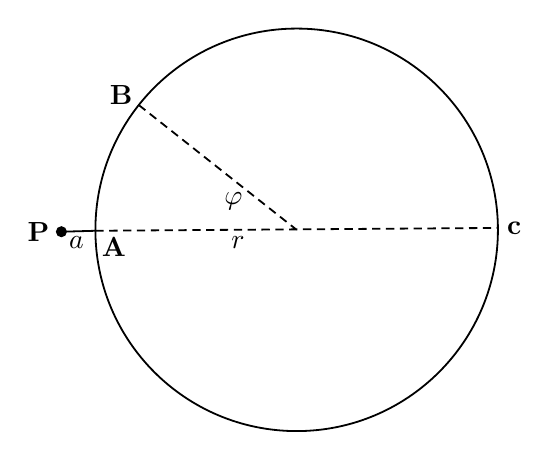
\begin{tikzpicture}[x=.12mm,y=.12mm,line width=.65pt]
  \coordinate (center) at (0,0);
  \coordinate (P) at (-249,-2);
  \coordinate (A) at (-213,-1);
  \coordinate (B) at (-167,132);
  \coordinate (c) at (213,2);
  \draw (center) circle[radius=25.56mm];
  \draw (P)--(A);
  \draw[dash pattern=on 3pt off 2pt] (A)--(c) (B)--(center);
  \fill (P) circle[radius=2pt];
  \node[left=4pt,inner sep=0pt] at (P) {\bfseries P};
  \node[anchor=north west,xshift=2pt,yshift=-2pt,inner sep=0pt] at (A) {\bfseries A};
  \node[anchor=south east,xshift=-2pt,inner sep=0pt] at (B) {\bfseries B};
  \node[right=3pt,inner sep=0pt] at (c) {\bfseries c};
  \node[below=2pt,inner sep=0pt] at (-233,0) {$a$};
  \node[below=2pt,inner sep=0pt] at (-62,0) {$r$};
  \node[above=1pt,inner sep=0pt] at (-67,17) {$\varphi$};
\end{tikzpicture}
\end{center}
\[
\begin{aligned}
&\text{1) through the portion }AB\,.\,.\text{ approximately }\log\frac{2r\sin\varphi}{a}\\
&\text{2) through the portion }BC\text{ approximately }-2-\log\operatorname{tg}\tfrac14\varphi\\
&\text{Combined}\quad\log\frac{8r\varphi}{a}-2=\log\frac{8r\varphi}{aee}\\
&\text{Through the entire circle}\quad2\log\frac{8r}{aee}
\end{aligned}
\]

\begin{center}[17.]\end{center}
Let a circle of radius $=\rho$ revolve about an axis in its plane, the center of the circle being at a distance $=R$ from the axis. Let the resulting ring-shaped solid region be filled uniformly with a rheophore circuit. Let the number of turns be $M$. Assume that $\rho$ is very small compared with $R$. The aim is to find the electromotive effect of the ring on a point either inside it or very close to it.
\begin{center}\begin{tikzpicture}[x=.12mm,y=.12mm,line width=.65pt]
  \coordinate (center) at (0,0);
  \coordinate (axisMid) at (525,0);
  \coordinate (axisTop) at (525,190);
  \coordinate (axisBottom) at (525,-167);
  \draw (center) circle[radius=16.32mm];
  \draw[dash pattern=on 3pt off 2pt] (center)--(axisMid) (axisTop)--(axisBottom);
\end{tikzpicture}
\end{center}

Let $a$ be the distance from the point to the centerline of the ring. The required effect is then
\[
\begin{aligned}
2M\log\frac{8R}{aee}&=2M\left\{\log\frac{8R}{a}-2\right\}\quad\text{if}\quad a>\rho\\
2M\left(\log\frac{8R}{\rho}-\tfrac32-\frac{aa}{2\rho\rho}\right)&\quad\text{if}\quad a<\rho
\end{aligned}
\]

\SourceLeaf{628}
The mean value for all points distributed uniformly \textit{inside} the ring is
\[
2M\left\{\log\frac{8R}{\rho}-\tfrac74\right\}
\]
or the total electromotive force experienced by a ring with $m$ turns, of the same shape as the inducing ring and acted on by it, is
\[
=4\pi mMR\left\{\log\frac{8R}{\rho}-\tfrac74\right\}=E
\]

For a given supply of wire for each circuit, $mR,MR$ and $\dfrac{m}{\rho\rho}$ are given. Since
\[
E=16\pi.\ MR.\ (mR)^{\frac23}.\ \left(\frac{m}{\rho\rho}\right)^{\frac13}.\ \left(\frac{8R}{\rho}\right)^{-\frac23}\left(\log\frac{8R}{\rho}-\tfrac74\right)
\]
for $E$ to reach \textit{a maximum},
\[
\left(\frac{8R}{\rho}\right)^{-\frac23}\left(\log\frac{8R}{\rho}-\tfrac74\right)
\]
must reach a maximum. Equivalently, with $\left(\dfrac{8R}{\rho}\right)^{\frac23}=x$,
\[
\frac{\log x^{\frac32}-\tfrac74}{x}=\tfrac32\left\{\frac{\log x-\tfrac76}{x}\right\}
\]
must reach a maximum.

This occurs when $\log x=\tfrac{13}{6}$
\[
\begin{aligned}
&\text{or}\quad\log\frac{8R}{\rho}=\tfrac{13}{4}\quad\text{is obtained}\\
&\text{or}\quad\log\operatorname{Brigg}\frac{8R}{\rho}=1{,}4114580\\
&\text{or}\quad\frac{8R}{\rho}=25{,}79\\
&\hphantom{\text{or}\quad}R=3{,}22\rho
\end{aligned}
\]

